\section{Models}
Here the basic definitions, the general models concept, and a list of
models available in \Dumux are given.

\subsection{Basic Definitions and Assumptions}
The basic definitions and assumptions are made, using the example
of a three-phase three-component system water-NAPL-gas
\cite{A3:class:2002a}. The modification for other multicomponent
systems is straightforward and can be found, e.\ g., in
\cite{A3:bielinski:2006,A3:acosta:2006}.

\begin{description}
\item[Components:]
The term \emph{component} stands for constituents of the phases which
can be associated with a unique chemical species, or, more generally, with
a group of species exploiting similar physical behavior. In this work, we
assume a water-gas-NAPL system composed of the phases water (subscript
$\text{w}$), gas ($\text{g}$), and NAPL ($\text{n}$). These phases are
composed of the components water (superscript $\text{w}$), the pseudo-component
air ($\text{a}$), and the organic contaminant ($\text{c}$) (see Fig.
\ref{fig:phaseMassEnergyTransfer}).

\item[Phases:]
For compositional multi-phase models, \emph{phases}
are not only matter of a single chemical substance. Instead, their
composition in general includes several species/components. For mass transfer,
the component behavior is quite different from the phase behavior.

\item[Equilibrium:]
For the non-isothermal, multi-phase, multi-component processes in porous media
we state that the assumption of \emph{local thermodynamic equilibrium}.
Chemical equilibrium means that the mass/mole fractions of a component in
different phases are in equilibrium.
Thermal equilibrium assumes the same temperature for all considered phases.
Mechanical equilibrium is not valid in a porous medium, since discontinuities
in pressure can occur across a fluid-fluid interface due to capillary effects.

\item[Notation:]
The subscript index $\alpha \in \{\text{w}, \text{n}, \text{g}\}$ refers
to the phase, while the superscript $\kappa \in \{\text{w}, \text{a}, \text{c}\}$
refers to the component.
\end{description}

\begin{table}
\begin{tabular}{llll}
$p_\alpha$ & phase pressure & $\phi$ & porosity \\
$T$ & temperature & $K$ & absolute permeability tensor \\
$S_\alpha$ & phase saturation & $\tau$ & tortuosity \\
$x_\alpha^\kappa$ & mole fraction of component $\kappa$ in phase $\alpha$ & $\boldsymbol{g}$ & gravitational acceleration \\
$X_\alpha^\kappa$ & mass fraction of component $\kappa$ in phase $\alpha$ & $q^\kappa_\alpha$ & volume source term of $\kappa$ in $\alpha$ \\
$\varrho_{\text{mol},\alpha}$ & molar density of phase $\alpha$ & $u_\alpha$ & specific internal energy \\
$\varrho_{\alpha}$ & mass density of phase $\alpha$ & $h_\alpha$ & specific enthalpy \\
$M$ & molar mass of a phase or component & $c_\text{s}$ & specific heat enthalpy \\
$k_{\text{r}\alpha}$ & relative permeability & $\lambda_\text{pm}$ & heat conductivity \\
$\mu_\alpha$ & phase viscosity & $q^h$ & heat source term \\
$D_\alpha^\kappa$ & diffusivity of component $\kappa$ in phase $\alpha$ & $\boldsymbol{v}_{a,\alpha}$  & advective velocity \\
$\boldsymbol{v}_\alpha$ & velocity (Darcy or free flow)& & \\
\end{tabular}
\caption{Notation list for most of the variables and indices used in \Dumux.}

\end{table}

\begin{figure}
  \centering
  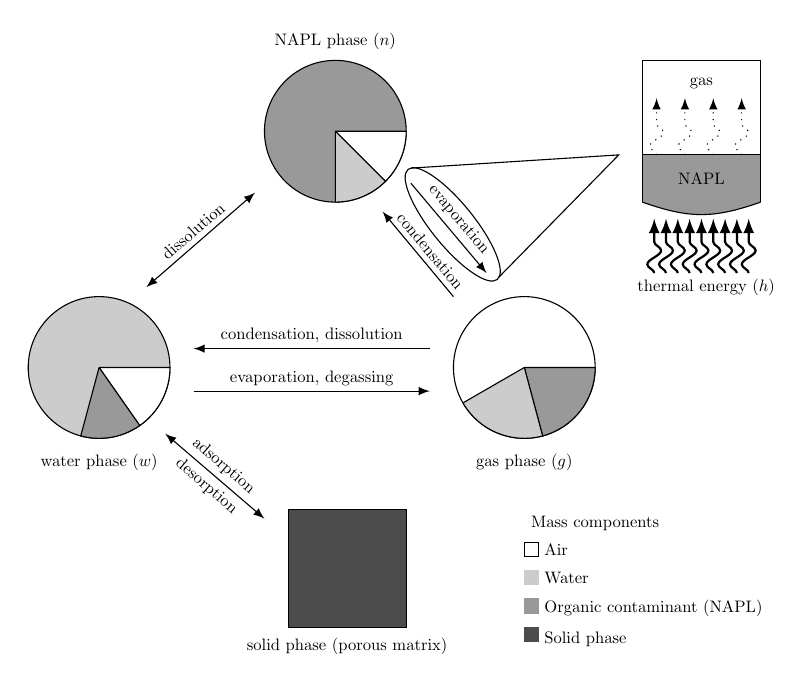
\begin{tikzpicture} [>=latex,scale=0.6, every node/.style={transform shape}]
    % Ellipse 1 solid
    \coordinate (A) at (1,-0.5);
    \draw [fill=black!70](A) rectangle(3.5,2) node at(2.25,-0.9) {solid phase (porous matrix)};
    % Ellipse 2 water
    \coordinate (B) at (-3,5);
    \draw [fill=black!20](B) circle(1.5cm);
    \node [yshift=5mm]at(-3,2.5){water phase $(w)$};
    \draw[fill=white] (B)--+(1.5,0)arc(0:-55:1.5cm)--(B);
    \draw[fill=black!40] (B)--+(-55:1.5cm)arc(-55:-105:1.5cm)--(B);
    % Ellipse 3 gas
    \coordinate (C) at (6,5);
    \draw [](C) circle (1.5cm);
    \node[yshift=5mm]at(6,2.5){gas phase $(g)$};
    \draw [fill=black!40](C)--+(1.5,0)arc(0:-75:1.5cm)--(C);
    \draw [fill=black!20] (C)--+(-75:1.5cm)arc(-75:-150:1.5cm)--(C);
    % Ellipse 4 napl
    \coordinate (D) at (2,10);
    \draw [fill=black!40](D) circle (1.5cm);
    \node[yshift=5mm]at(2,11.4){NAPL phase $(n)$};
    \draw [fill=white](D)--+(1.5,0)arc(0:-45:1.5cm)--(D);
    \draw [fill=black!20] (D)--+(0,-1.5)arc(-90:-45:1.5cm)--(D);
    % arrows
    %A-B
      \draw [<->,white](0.5,1.8)--(-1.6,3.6) node[black,above,sloped,pos=0.5]{adsorption};
      \draw [<->](0.5,1.8)--(-1.6,3.6) node[below,sloped,pos=0.5]{desorption};
    %B-C
      \draw[<-](-1,5.4)--(4,5.4)node[above,sloped,pos=0.5]{condensation, dissolution};
      \draw[->](-1,4.5)--(4,4.5)node[above,sloped,pos=0.5]{evaporation, degassing};
    %B-D
      \draw[<->](-2,6.7)--(0.3,8.7)node[above,sloped,pos=0.5]{dissolution};
    %D-C
      \draw[->](3.6,8.9)--(5.2,7)node[above,sloped,pos=0.5]{evaporation};
      \draw[rotate around={-51:(4,6.8)}](3.35,7.95) ellipse (1.5cm and 0.45cm);  %Ellipse um evaporation
      \draw (3.6,9.22)--(8,9.5)--(5.45,6.9);
      \draw[<-](3,8.3)--(4.5,6.5)node[above,sloped,pos=0.55]{condensation};
    % thermal energy
    \filldraw [black!40](8.5,9.5)rectangle(11,8.5);
    \draw (8.5,9.5)rectangle(11,11.5);
    \draw (8.5,9.5)--(8.5,8.5);
    \draw (11,9.5)--(11,8.5);
    \draw [decorate,decoration={bent,aspect=0.4,amplitude=6},fill=black!40](11,8.5)--(8.5,8.5);
    \foreach \x in {8.75,9,...,10.8}
    \draw [->,decorate,decoration={snake,post length=2mm},thick](\x,7)--(\x,8.15);
    \foreach \x in {8.8,9.4,10,10.6}
    \draw [->,dotted,decorate,decoration={snake,post length=2mm}](\x,9.5)--(\x,10.7);
    \node at(9.75,11){gas};
    \node at(9.75,9){NAPL};
    \node at(9.85,6.7){thermal energy $(h)$};
    % legende
    \node at (7.5,1.7){Mass components};
    \draw[](6,1)rectangle +(0.3,0.3) node at(6.3,1.15) [right]{Air};
    \filldraw[black!20](6,0.4) rectangle +(0.3,0.3) node at (6.3,0.55)[black,right]{Water};
    \filldraw[black!40](6,-0.2) rectangle +(0.3,0.3) node at (6.3,-0.1)[right,black]{Organic contaminant (NAPL)};
    \filldraw[black!70](6,-0.8) rectangle +(0.3,0.3) node at (6.3,-0.75)[right,black]{Solid phase};
  \end{tikzpicture}
  \caption{Mass and energy transfer between the phases}
  \label{fig:phaseMassEnergyTransfer}
\end{figure}



\subsection{Available Models}
We distinguish fully-implicit and sequential models. A list of all available models can be found
in the Doxygen documentation at
\url{http://www.dumux.org/doxygen-stable/html-\DumuxVersion/modules.php}.
The documentation includes a detailed description for every model.

\subsubsection{Fully-Implicit Models}
The fully-implicit models are using the box or the
cell-centered finite volume method as described in section \ref{box} and \ref{cc}
for spatial and the implicit Euler
method as temporal discretization. The fully-implicit models are located in
subdirectories of \texttt{dumux/freeflow}, \texttt{dumux/geomechanics}, 
and \texttt{dumux/porousmediumflow}.

Grid adaption is available for both discretization schemes, box and cc.  The \texttt{adaptionhelper}-method has to be adjusted to the respective model.
Note that the current implementation only ensures mass conservation for incompressible fluids.
In general, the spatial  parameters, especially the porosity, have to be assigned on
the coarsest level of discretization.

\subsubsection{Sequential Models}
The basic idea of the sequential models is to reformulate the
equations of multi-phase flow into one equation for
pressure and equations for phase/component/... transport. The pressure equation
is the sum of the mass balance equations and thus considers the total flow of the
fluid system. The new set of equations is considered as decoupled (or weakly coupled)
and can thus be solved sequentially. The most popular sequential model is the
fractional flow formulation for two-phase flow which is usually implemented applying
an IMplicit Pressure Explicit Saturation algorithm (IMPES).
In comparison to a fully implicit model, the sequential structure allows the use of
different discretization methods for the different equations. The standard method
used in the sequential models is a cell-centered finite volume method. Further schemes,
so far only available for the two-phase pressure equation, are cell-centered finite
volumes with multi-point flux approximation (MPFA O-method) and mimetic finite differences.

An $h$-adaptive implementation of both sequential models is provided for two dimensions.
The sequential models are located in
subdirectories of \texttt{dumux/porousmediumflow}.
